\chapter{Literature Review}\label{ch:methodology}

\section{Medical Background of Esophageal Swallowing}

Swallowing is a complex but orderly physiological process transporting saliva or food from the mouth to the stomach. The swallowing physiology and anatomy are elucidated with the critical insights from the in vivo studies \citep{Dodds1989}. Any esophageal impairment compromises the efficiency of swallowing, is known as dysphagia \citep{Groher2015}. Severe pathologies, for instance, benign esophageal strictures from various injuries, esophageal cancer, and esophageal perforations, distressing lumen patency explicitly leading to dysphagia. Unaccompanied by comprehensive care, a vicious cycle materializes as malnutrition and dehydration aggravating the dysphagia itself, subsequently increasing morbidity and even mortality \citep{Garcia2010}. The standard clinical practices involve evaluation of the etiology of the swallowing deficit using perception studies, and in vivo analysis, followed by intervention strategies for nutritional support \citep{Kuo2012}. Depending upon the severity, the method of maintaining nutrition varies from oral dietary supplements, texture modified foods, implanting nasogastric feeding tubes, surgical correction, endoscopic dilation of the sphincters, and esophageal stenting \cite{Groher2015,Cichero2017}.

\subsection{Swallowing Process}
The anatomy of the human digestive system begins with munching, mashing, and mixing the food in the mouth and ends at the anus (\autoref{fig1_Dig_sys}). The process of swallowing, which is sometimes referred to as deglutition, involves transportation of food bolus from the oral cavity to the stomach through the esophagus with the aid of peristaltic waves in the esophageal conduit, generated by central pattern generators (CPGs). 
The desired result of swallowing is not only the successful transportation of food but also the removal of the food particles from the respiratory tract so that the respiratory tract does not ingest any unwanted particles. \cite{Miller1986,Miller1987,lang2009brain}. 

\begin{figure}[bth]
	\myfloatalign
	{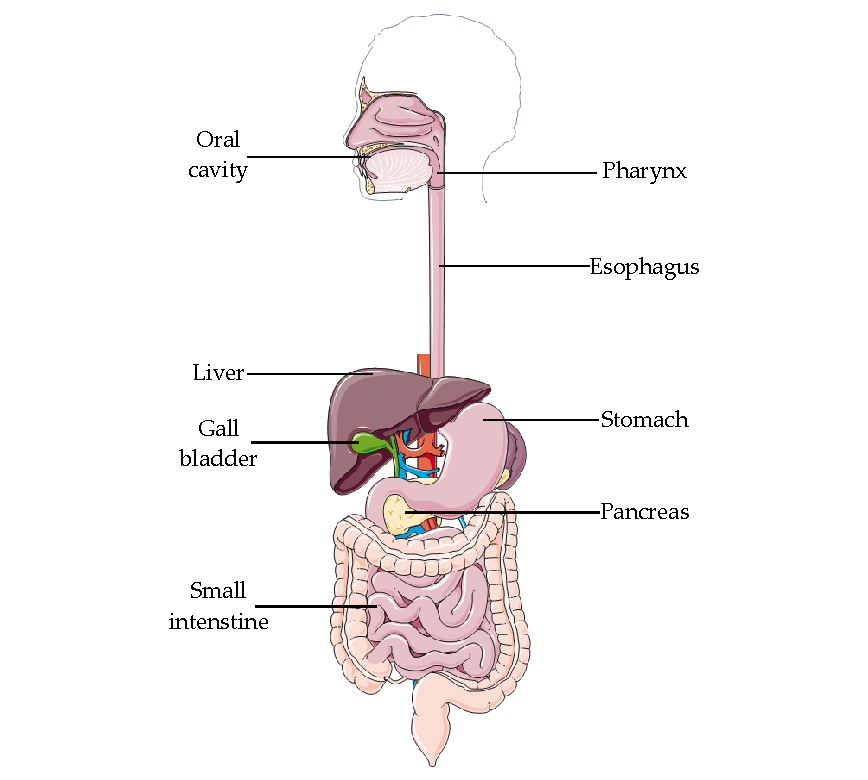
\includegraphics[width=\linewidth]{images/Ch2/fig1_Dig_sys}} \quad
	\caption[Anatomy of human digestive system.]{Anatomy of human digestive system.}\label{fig1_Dig_sys}
\end{figure}

\subsection{Stages of swallowing}
The neurophysiological control of the swallowing process comprises of three distinct phases where each phase is interacting with each other. The degree of dependence of each stage on the neuron control varies in each phase  \citep{lang2009brain}.

\subsubsection{Oral preparatory stage}
The oral preparatory phase is responsible for the primary preparation of the food bolus before the bolus enters the pharynx. After the mastication, it breaks down the ingested food in sufficiently small sizes and mixes it well with the saliva for transport through the pharynx and esophagus for digestion within the stomach \citep{Miller1986}.

\subsubsection{Pharyngeal stage}
The pharyngeal stage does the propelling of the food bolus to the esophagus. While doing the transport, it consistently coordinates with the respiratory tract so that it can be protected from the unwanted food particles. Four major activities done by the pharyngeal stage are \citep{Miller1986}. 

\begin{itemize}
	\item  Propelling the food bolus.
	\item  Inhibition of respiration
	\item  Closure of the palatopharyngeal isthmus
	\item  Constiction of the larynx    
\end{itemize}

\subsubsection{Esophageal stage}

The esophageal stage follows the pharyngeal stage, but it can function completely independent of any other stages of swallowing and has its own distinct neural control \cite{Miller1986, Miller1987, lang2009brain, Dodds1989}. The esophagus (Latin: \textit{oesophagus}), 180 to 260 mm in length, consists of a muscular tube that spans rostral caudally from the pharynx in the upper aspect, down to the stomach whose elementary function is to push the swallowed food and fluid from the oral cavity to the stomach by peristaltic contractions (\autoref{fig1_Dig_sys}) \cite{brasseur1987fluid,Miller1986,chen2009food}. 


\begin{figure}[bth]
	\myfloatalign
	{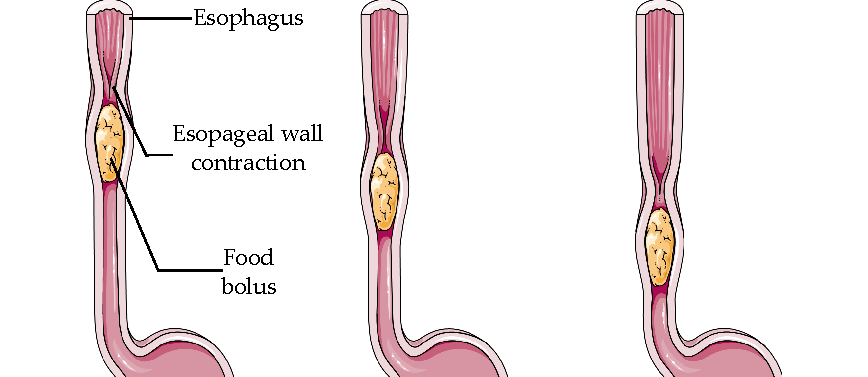
\includegraphics[width=\linewidth]{images/Ch2/fig2_Peristalsis}} \quad
	\caption[Esophageal peristalsis]{Esophageal peristalsis. The process of swallowing involves transportation of food bolus from the oral cavity to the stomach through the esophagus with the aid of esophageal wall contractions generated by spatio-temporal peristaltic waves.}\label{fig2_Peristalsis}
\end{figure}

\autoref{tab1_esophagus} summarizes all the relevant attributes of the human esophagus. The esophageal wall is made up of mucosa, submucosa and muscularis propria. The muscularis propria consists of outer longitudinal and inner circular muscle fibers, which activates sequentially to generate an esophageal wall contraction behind the bolus (\autoref{fig2_Peristalsis}) \cite{brasseur1987fluid,Miller1986,Miller1987,Dodds1989}. The fast movement of the bolus does not occur in the supine position, which evident the fact that bolus velocity is mostly governed by gravity \cite{mashimo2006physiology,brasseur1987fluid}. However, it has been shown that the process does not depend on gravity for
transport, as swallowing can be conducted in an inverted person \cite{chen2009food}. 

\begin{table}
	\myfloatalign
		\caption[Attributes of human esophagus and esophageal peristaltic transport.]{Attributes of human esophagus and esophageal peristaltic transport.}  \label{tab1_esophagus}
	\begin{tabularx}{\textwidth}{Xl} \toprule
		\tableheadline{Esophagus quantitative attributes}\\
		\midrule
		\tableheadline{Attribute} & \tableheadline{Magnitude} \\ \midrule
		Esophagus conduit length & 180 - 260 mm  \cite{brasseur1987fluid,Dodds1989}\\
		Conduit diameter & 20 - 23 mm \\
		Peristalsis wave velocity & 20 - 40 mms$^{-1}$  \cite{brasseur1987fluid,Jean2001}\\
		Wavefront length & 30 - 60 mm \\
		Wave seal pressure & 15 KPa  \cite{brasseur1987fluid}\\
		\midrule
		\tableheadline{Esophagus qualitative attributes}\\
		\midrule
		\tableheadline{Attribute} & \tableheadline{Behavior} \\ \midrule
		Wall material composition &  \multirow{2}{*}{\begin{tabular}[c]{@{}l@{}}Mucosa, submucosa,\\ and muscularis propria \citep{mashimo2006physiology}\end{tabular}} \\
		& \\
		Wall material feature & Compliant, and continuous\\
		Muscle fiber type & Longitudnal, and circular  \citep{mashimo2006physiology}\\
		Muscle distribution & Striated, and smooth \citep{mashimo2006physiology}\\
		Transport type & Peristaltic \cite{ghosh2006physiology}\\
		Wave shape & Sinusoidal  \\
		\midrule
		\tableheadline{Peristalsis attributes} \cite{ghosh2006physiology, Dodds1989, lang2009brain}\\
		\midrule
		Peristalsis type & Primary, and secondary\\
		Primary peristalsis (\ac{PP}) location & Smooth, and striated\\
		Primary peristalsis mechanism & Central\\
		Secondary peristalsis (\ac {SP}) location & Elicited from incomplete \ac{PP}\\
		
		\bottomrule
	\end{tabularx}

\end{table}

\subsubsection{Swallowing Mechanism}


Videofluoroscopy, and manometry techniques are used hand in hand to determine the \ac{ILPS}. In an esophageal peristaltic transport of food bolus, the manometry and videofluoroscopic recordings can be distributed into two \ac{ILPS} segments (\autoref{fig4_BolusPressureSig}) \cite{brasseur1987fluid,ren1993determinants,ghosh2006physiology}. In the first segment, within the bolus fluid, the recorded pressure is solely due to the hydrodynamic bolus pressure, which is also known as the \ac{IBPS}. At the tip of the bolus tail, the pressure undergoes a transition from \ac{IBPS} to esophageal direct contact pressure with the manometry catheter, which can be regarded as the second segment. The contact pressure is the \ac{PILPS}, which reflects the maximum esophageal muscle squeeze pressure aboove the bolus tail \citep{ghosh2006physiology}. The \ac{MIBPS} occurs at the bolus tail tip, and after which, no bolus fluid exists, leading to direct contact pressure. Since pressure cannot be transmitted axially in the absence of bolus fluid; thus, these two segments are independent of each other \cite{brasseur1987fluid}.  

\begin{figure}[bth]
	\myfloatalign
	{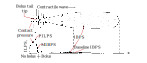
\includegraphics[width=\linewidth]{images/Ch2/fig4_BolusPressureSig}} \quad
	\caption[Schematic of axial distribution of intraluminal pressure signature  (ILPS) in an esophagus.]{Schematic of axial distribution of Intraluminal Pressure Signature  (ILPS) in an esophagus \cite{brasseur1987fluid}.}\label{fig4_BolusPressureSig}
\end{figure}

A dry swallow is an act of swallowing something without the aid of any liquid like water. It is associated with the swallowing of the air bolus. As there is no bolus present, hence there is no distension on the muscle of the esophagus, which results in the generation of low \ac{PILPS} waves \cite{hollis1975effect}. Wet swallows associated with liquid bolus of lower volume (<1 ml) have exhibited lower \ac{PILPS}, similar to dry swallows. However, wet swallows of bolus volume greater than 2 ml, have shown higher \ac{PILPS}, slower wave speed, and greater contraction wave duration as compared to low volume bolus. Besides, the strength of the esophageal contractions depicted by \ac{PILPS}, remains the same for all bolus volume higher than 2 ml, which indicates the fact that a critical bolus volume is required to initiate \ac{PP}. Additionally, \ac{PILPS} of the contraction waves and other parameters cannot be consciunsupersly altered \cite{hollis1975effect}. 

The \ac{IBPS} remains almost equal throughout the length of the esophagus but, \ac{IBPS} increases with bolus volume and bolus viscosity. Additionally, the dependence of \ac{IBPS} on bolus viscosity is only significant for bolus volume above 10 ml. Similarly, bolus transit time also does not vary throughout the esophagus, and it is independent of bolus volume and viscosity. 

A successful transit of the bolus is referred to as effective
peristalsis while, ineffective peristalsis is often associated with
the residue of food particles left in the esophagus \citep{ghosh2006physiology}. In an effective bolus transport, maximum intraluminal cross-sectional diameter generally increases as the bolus moves distally. While, increase in bolus volume significantly increases the diameter, the increase in viscosity have not shown any significant impact on it \cite{ren1993determinants}. For an ineffective peristalsis, when the esophageal muscular contractions are not enough to occlude the esophagus, the magnitude of \ac{MIBPS} remains closer to \ac{PILPS}. For a succesful bolus transport, \ac{PILPS}-\ac{BIBPS} $  \ge$ 2.7 KPa (20 mmHG) \cite{ren1993determinants,ghosh2006physiology}. The relation is independent of all bolus viscosity and volume and if the difference is below 2.7 KPa, the chances of ineffective peristalsis increases further. Hence, determining the pressure difference can be a useful tool to assess the peristaltic transport failure.

\subsection{Swallowing Peristalsis}
The muscularis propria () is predominantly comprises of striated muscle in proximal one-third of the esophagus and smooth muscle in the distal two-thirds of the esophagus (\autoref{fig3_EsophagusMuscle},\autoref{tab1_esophagus}) \citep{ghosh2006physiology,mashimo2006physiology}. Recent experiments were conducted by \ac{HRM} have shown that the peristalsis associated with the esophagus involves two different types of contractile waves, conforming to separate muscle kinds (striated and smooth) and neuronal control systems of the proximal and distal esophagus \cite{Crist1984,jeong2014utilizing,ghosh2006physiology}. With computer simulations, Li et al. \cite{Li1994Analyses} reported the existence of two seperate contraction waves in the \ac{ROT} from striated to smooth muscle, separated by > 4 cm, to explain the pressure measurememnt due to bolus retention in that region. Additionally, they also reported a space-time coordination between the two waves across the transition region to clear the bolus effectively (\autoref{tab1_esophagus}). The two types of peristaltic contraction waves, which occur on the wall of the esophagus are:

\begin{figure}[bth]
	\myfloatalign
	{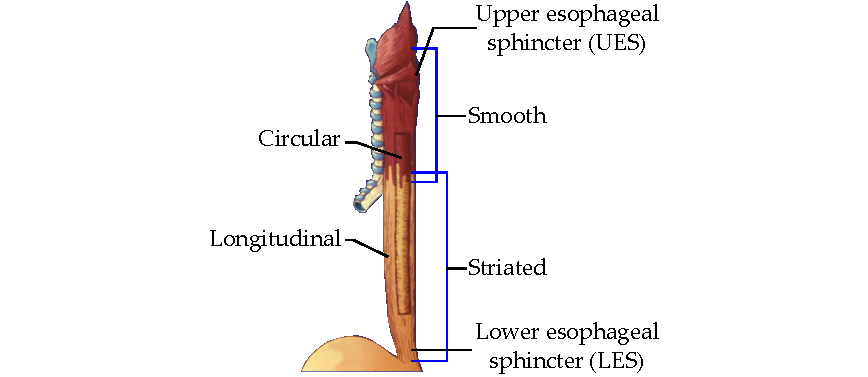
\includegraphics[width=\linewidth]{images/Ch2/fig3_EsophagusMuscle}} \quad
	\caption[Muscular anatomy of esophagus]{Muscular anatomy of esophagus. \citep{mashimo2006physiology}}\label{fig3_EsophagusMuscle}
\end{figure}

\begin{itemize}
	\item Primary peristalsis
	
	\ac{PP} is a voluntary contraction that can occur due to the stimulation of the receptive fields in the esophagus. The primary peristalsis mostly takes place in both striated and smooth muscle fibers. In striated muscle fibers, the peristalsis is controlled by the central swallowing program (neural excitation) (\autoref{tab1_esophagus}) \cite{Dodds1989}.
	
	\item Secondary peristalsis
	
	
	\ac{SP} arises whenever there is a bolus remaining in the esophagus in which stimulus to the oesophageal receptive fields initiates the peristalsis. The peristaltic wave can be activated by the distension of any part of the esophagus (\autoref{tab1_esophagus}) \cite{lang2009brain}.
\end{itemize}

Ghosh et al. \cite{ghosh2006physiology} analysed the \ac{ROT} using \ac{HRM} and digital fluoroscopy. During \ac{PPW} propagation, \ac{PILPS} follows the bolus tail and for successful bolus transport it remains higher than \ac{MIBPS} ($t_1$). As soon as \ac{PPW} enters the ROT ($ t_2$), it starts to slow down, and \ac{PILPS} decreases and hence, esophageal muscle squeeze reduces ($ t_2$ to $t_3$). Concurrently, another wave known as the \ac{IW} begins to compensate the \ac{PPW}. As, IW progresses, it occludes the lumen increasingly ($ t_3$ to $t_5 $) and \ac{PILPS} shifts in front of \ac{MIBPS} ($ t_5 $). IW travels until it fully occludes the lumen ($ t_6$ to $t_7$), and initiates the beginning of \ac{SPW} ($ t_7 $). Concurrently, the \ac{PPW} ends and birth of a new bolus tail takes place. Since for a successful bolus transport, \ac{PILPS} must be higher than \ac{MIBPS}; thus  \ac{MIBPS} jumps ($ t_7$ to $t_8 $). 

\begin{figure}[bth]
	\myfloatalign
	{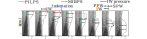
\includegraphics[width=\linewidth]{images/Ch2/fig5_ROT}} \quad
	\caption[Pressure signature and bolus coordination during bolus transport through the Region of Transition (ROT) in a normal subject.]{Pressure signature and bolus coordination during bolus transport through the ROT in a normal subject. \citep{ghosh2006physiology}}\label{fig5_ROT}
\end{figure}

\autoref{tab1_peristalsis} summarizes the effect of different bolus types and bolus volume on the \ac{PILPS}, \ac{MIBPS}, and \ac{BIBPS}. 
\newgeometry{margin=1mm} % modify this if you need even more space
\begin{landscape}
	{\footnotesize
		\vspace*{\fill}
		\vspace*{\fill}
		\vspace*{\fill}
		\begin{longtable}{llllllllll} 
		\caption{Effect of different bolus types and bolus volume on the pressure signature generated by peristaltic waves.}\label{tab1_peristalsis}\\\toprule
Characteristics                                                                                                                                                                                                                    & Bolus attributes                                                                       & \multicolumn{3}{c}{\begin{tabular}[c]{@{}c@{}}Pressure amplitude\\ (mmHg)\end{tabular}}                                               & \begin{tabular}[c]{@{}c@{}}Mean velocity\\ (mms$-1$)\end{tabular} & Ref.      \\
\midrule
&                                                                                    & Upper                                                     & Middle (ROT)                                          & Lower    &                                                           &          \\
\midrule


\multirow{4}{*}{\begin{tabular}[c]{@{}l@{}}The act of swallowing can initiate peristalsis. \\ Food bolus volume, and viscosity can regulate peristalsis.\end{tabular}}                                                          & Dry                                                                                &PILPS = 49 $\pm$ 7.5 &PILPS = 70 $\pm$ 10.7 &          &40.85 $\pm$ 3.6 &  \\
& 1 ml                                                                               &PILPS = 61 $\pm$ 7.5       &PILPS = 66 $\pm$ 6.7&          & 33 $\pm$ 1.9          &   \cite{hollis1975effect}       \\
& 20 ml                                                                              &PILPS = 107 $\pm$ 13     &PILPS = 127 $\pm$ 15.7&          &                                                                 &          \\
\midrule

\multirow{3}{*}{\begin{tabular}[c]{@{}l@{}}PILPS - BIBPS $\ge$ 20 mmHg (2.7 KPa).\\ BIBPS independent of manometric location without \ac{AC}.\\ BIBPS increases at distal part with AC.\\ BIBPS increases with volume and viscosity ($\ge$ 10 ml).\end{tabular}} &  10 ml without AC & \multicolumn{3}{c}{--BIBPS = 12--}                                                                                             &       35.85 $\pm$ 2.0                                                          &                        \\
& 20 ml without AC & \multicolumn{3}{c}{--BIBPS = 15--}                                                                                             &     35.85 $\pm$ 2.0                                                            & \cite{ren1993determinants}                          \\
& 10 ml with AC                                                                      &  BIBPS = 12.0                                                      & BIBPS = 12.0                     & BIBPS = 28.0                       &                                                                 &                           \\                                                                   & 20 ml with AC                                                                      &  BIBPS = 15.0                                                      & BIBPS = 15.0                     & BIBPS = 28.0                       &                                                                 &                           \\                                                                                                                                                                &                                                                                    &\\ 
\midrule



\multirow{6}{*}{Dysphagia patients suffering from Achalasia or Chagas disease.}                                                                                                                                                                                                                 & Dry swallow (Normal)                    & PILPS = 78.7                                                      & PILPS = 45                                                    &          &                                                                 &          \\
& Wet swallow (Normal)                   & PILPS = 95.1                                                      & PILPS = 88.3                                                  &          &                                                                 &          \\
& Dry swallow (Achalasia)       & PILPS = 32.4                                                      & PILPS = 46.1                                                  &          &                                                                 &          \cite{dalmazo2010esophageal}\\
& Wet swallow (Achalasia)               & PILPS = 31.4                                                      & PILPS = 38.9                                                  &          &                                                                 &          \\
& Dry swallow (Chagas)                  & PILPS = 63.8                                                      & PILPS = 24.7                                                  &          &                                                                 &          \\
& Wet swallow (Chagas)             & 75.4                                                      & PILPS = 37.2                                                  &          &                                                                 & \\
\midrule


\multirow{3}{*}{\begin{tabular}[c]{@{}l@{}}Mean velocity of the wave increases from upper to distal part of the esophagus.\\ A significant reduction in the rate of pressure was found in the upper esophagus.\end{tabular}}       & Wet swallow                                                                        & \multicolumn{1}{l}{PILPS = 53.4}                          & \multicolumn{1}{l}{PILPS = 35.0}                        & \multicolumn{1}{l}{PILPS = 69.5} & \multicolumn{1}{l}{}                                            & \multicolumn{1}{l}{} \\
&                                                                                    & \multicolumn{1}{l}{}                                      & \multicolumn{1}{l}{}                                  & \multicolumn{1}{l}{}             & \multicolumn{1}{l}{}                                            & \multicolumn{1}{l}{\cite{dalmazo2010esophageal}} \\
&                                                                                    & \multicolumn{1}{l}{}                                      & \multicolumn{1}{l}{}                                  & \multicolumn{1}{l}{}             & \multicolumn{1}{l}{}                                            & \multicolumn{1}{l}{}\\
\midrule


\begin{tabular}[c]{@{}l@{}}Transition from PPW to SPW occurs in the ROT.\\ Spatial jump of PPW to SPW in the ROT.\end{tabular}                                                                                                    & Bolus swallow                                                                      & \multicolumn{1}{l}{}                 & \multicolumn{1}{l}{\begin{tabular}[c]{@{}l@{}}PILPS=46.5 $\pm$ 12.4\\ MIBPS=32.1 $\pm$ 11.9\end{tabular}}           & \multicolumn{1}{l}{}             & \multicolumn{1}{l}{}                                            & \multicolumn{1}{l}{\cite{clouse1996characteristics}}\\\bottomrule
  
	\end{longtable}}
\end{landscape}

\restoregeometry
\thispagestyle{empty} 


The shortcomings of these techniques are X-ray radiation exposure and catheterization (inserting a manometry catheter) that accumulate to the efforts of swallowing and the general health of subjected individuals.[Roy]

\subsection{Neuronal Circuits of Swallowing: Central Pattern Generators (CPGs)}

The esophageal stage of swallowing, although connected to the pharyngeal stage, is following its own distinctly separate neural control. The \ac{PP} occurs deliberately with the stimulation of receptive territories in the oropharyngeal range, while \ac{SP} happens if bolus or a part of the bolus gets stuck in the esophagus in which stimulation to the oesophageal receptive territories begins the peristalsis \cite{Miller1986,Miller1987}. There are many mechanisms to coordinate the esophageal swallowing process, primarily controlled by both brain stem control and external coordination control. The brain stem control is triggered by patterns of neural or declining cortical input. The findings of \cite{Miller1986,Miller1987}, also support the fact that the contraction of the entire esophagus takes place, which includes both the smooth and striated muscle fibers during \ac{PP}. \ac{PP} is associated with the swallowing, and it is centrally controlled by the activation of the motor neurons \cite{Miller1986,Miller1987}.

The brain stem control consists of three parts for controlling the esophageal swallowing, the \ac{CPG}, pre-motor circuitry, and motor neurons \cite{lang2009brain}. Studies in electrophysiology conducted by Jean \cite{Jean2001,jean1972localization} have proved the existence of the timing pattern generator circuits. The events caused by these generators are natural and local in nature, such that the feedback from the periphery does not affect the generation of the patterns because they persist even in paralyzed animals \cite{jean1972localization}. In other words, it can be written that the pattern generators govern the sequence of the motor responses in the esophageal swallowing process.

The microelectrode experiments conducted by Jean \cite{Jean2001}, showed that the swallowing \ac{CPG} includes two major neuron groups. One group is located in the nucleus tractus solitarii of the dorsal medulla and held responsible for pattern generation and their characteristics like time of triggering, shaping and timing of the rhythmic pattern. The second group is in the ventrolateral medulla, which divides the swallowing drive to the different pools of motor neurons included in swallowing.
The threshold that induces the swallowing depends upon many factors like the type of fluids, touch, the pressure exerted by the food bolus, and range of salivation. By having a sensory feedback mechanism, the threshold and intensity of sequential muscle requirement for the peristalsis can be changed \cite{Miller1987}. Inter and intra-form of reflexes also change or adjust the swallowing to consider the alterations in physiologic functions. These alterations combine the deglutitory inhibition, failed swallow, and \ac{SP} \cite{lang2009brain}.

\subsection{Dysphagia}

The primary purpose of the esophagus is to deliver the food from the mouth to the stomach. Complete food bolus transit is referred to as a successful swallow, and it is associated with effective peristalsis. An ineffective peristaltic wave often leads to a residue of food particles left in the esophagus \cite{ren1993determinants}. 

Any esophageal impairment compromises the efficiency of swallowing, is known as dysphagia \cite{Dodds1989}. Severe pathologies, for instance, benign esophageal strictures from various injuries, esophageal cancer, and esophageal perforations, distressing lumen patency explicitly leading to dysphagia. Unaccompanied by comprehensive care, a vicious cycle materializes as malnutrition and dehydration aggravating the dysphagia itself, subsequently increasing morbidity and even mortality \cite{Groher2015}. The standard clinical practices involve evaluation of the etiology of the swallowing deficit using perception studies, and in vivo analysis, followed by intervention strategies for nutritional support \cite{Kuo2012}. Depending upon the severity, the method of maintaining nutrition, varies from oral dietary supplements, texture modified foods, implanting nasogastric feeding tubes, surgical correction, endoscopic dilation of the sphincters, and esophageal stenting \cite{Groher2015,Cichero2017}.


The estimates show that dysphagia affects one-twelfth of the world's population. Different texture modifications on food like chopping, mashing, and pureeing on food are done across the globe so that the swallowing process in dysphagic patients can be improved. Liquids are often thickened to increase the swallowing time \cite{Cichero2017}. It's highly challenging for such patients to chew and swallow food having high Young's modulus. By introducing some modifications to the food, the effort required for swallowing can be significantly reduced, and it can add nutritional value to their daily oral food intake as well. 

Dysphagia patients often suffer from conditions leading to ineffective peristalsis, and hence remaining residue of food particles in the esophagus \cite{Carrier2007Cognitive}.  For a successful swallow, the intraluminal and the intrabolus pressure must overcome the obstruction created by the esophagogastric junction \cite{jeong2014utilizing,ren1993determinants}. It is often seen that wet and bolus swallows comparatively causes the higher strength of contraction waves (higher \ac{PILPS}) in the distal part of the esophagus than dry swallows. This phenomenon is not observed in the subjects suffering from diseases like achalasia and Chagas disease due to the impairment of the oesophageal nervous system abnormalities. Such kind of nervous abnormalities causes alterations in the motility of the esophagus \cite{dalmazo2010esophageal}.

\section{Stretchable and Flexible Sensors}

Sensors made from stretchable materials could be incorporated into soft robots for sensing its different elements. Due to their flexibility and transparency, sensors manufactured from \ac{CNT}, graphene, and \ac{SNT} have gained much significant attention for application in flexible electronics and the field of robotics. Instead of developing new materials, conventional rigid materials such as silicon and allotropes of carbon are engineered to prepare these sensors.  The principle behind the working of these sensors is when the nanotubes are stretched, gaps and islands are formed on the films of these tubes due to fracture and bundle formation take place, which bridges the gap. This allows the nanotubes to act as strain sensors. By employing different manufacturing processes, the properties of the materials can be differed depending on the type of application. High durability, fast response, and low creep are some of the advantages of soft sensors over their rigid counterparts. \ac{CNT} sensors are popular due to their low cost, linearity and chemical stability. The in-plane strain sensors built from \ac{CNT} exhibits a high piezoresistive response \cite{Miao2011Optimization,miao2012modelling}, but extensive use of these sensors makes the nanotubes buckle due to the release of load, and the effect is known as buckling effect which leads to a wavy structure \cite{Shi2016Graphene}. By filling graphene into the nanotubes, voids can improve the strength of nanotubes significantly, and buckling can be prevented while maintaining the transparency of the material. Table 6and Table 7 summarises some of the \ac{CNT}-based sensors, their characteristics, and their application.

\newgeometry{margin=1mm} % modify this if you need even more space
\begin{landscape}
	{\footnotesize
		\vspace*{\fill}
		\vspace*{\fill}
		\vspace*{\fill}
		\begin{longtable}{llllll} 
		\caption{Different stretchable and flexible sensors, their constructions, advantages, and applications.}\label{tab1_peristalsis}\\\toprule
Name&Materials&Methods&Advantages&Applications&Ref.\\ 
\midrule                                              
\multirow{3}{*}{\begin{tabular}[c]{@{}l@{}}\ac{CNT} embroidered \\graphene (CeG)\end{tabular}}& & Hybridized film of \ac{CNT} and graphene&Increases strength at the nanotubes joints.&&\\
&\ac{CNT} graphene& Chemical vapour deposition (CVD) &Prevention of buckling behaviour.& {\begin{tabular}[c]{@{}l@{}}Motion sensing \\applications (\autoref{fig6_Sensors}a).\end{tabular}}&\cite{Shi2016Graphene}\\
&& \ac{PDMS} was used. &Linear and positive resistance change.&&\\
\midrule                                              
\multirow{3}{*}{CNT film strain sensor} & \multirow{3}{*}{\begin{tabular}[c]{@{}l@{}}Single-walled \ac{CNT} \\ (SWCNT) thin films\end{tabular}} & \multirow{3}{*}{\begin{tabular}[c]{@{}l@{}}Individually removed and laid side by side, \\ with a 1 mm overlap, onto \ac{PDMS}\end{tabular}} & High selectivity against twist.                                                                                                                    &  &          \\
&                                                                                                  &                                                                                                                                        & High durability and reproducibility.                                                                                                                               & {\begin{tabular}[c]{@{}l@{}}Human motion \\detection (\autoref{fig6_Sensors}b,c, and e).\end{tabular}} & \cite{Yamada2011Stretchable} \\
&                                                                                                  &                                                                                                                                        & \begin{tabular}[c]{@{}l@{}}The response of the \ac{CNT} strain sensor \\ to the strain is fast, with a low \\overshoot of 3.0 \% and recovery.\end{tabular} &  &\\

\midrule



\multirow{4}{*}{\begin{tabular}[c]{@{}l@{}}Graphene Porous\\ Network (GPN) - PDMS\end{tabular}} & \multirow{4}{*}{\begin{tabular}[c]{@{}l@{}}Nickel,\\ Graphene\end{tabular}} & Graphene growth.        &                                                                                       & Finger motion.          & \multirow{4}{*}{\cite{pang2016flexible}} \\
&                                                                             & \ac{PDMS} infilteration.& Wide pressure sensing range.                                                          & Blood pressure monitor. &                           \\
&                                                                             & Cutting redundant PDMS. & \begin{tabular}[c]{@{}l@{}}Highest sensitivity among\\ graphene sensors.\end{tabular} & Walking state.          &                           \\
&                                                                             & Ni etching.             &                                                                                       & Degree of finger blood. &               \\\midrule





\multirow{3}{*}{\begin{tabular}[c]{@{}l@{}}Dynamically stretchable\\ solid state supercapacitor\\ using graphene woven fabric (GWF)\end{tabular}} & Polyaniline                                                              & Stretching \ac{PDMS}                & \multirow{3}{*}{\begin{tabular}[c]{@{}l@{}}Excellent stretch ability under\\ high strain.\end{tabular}} & Wearable electronics                                                                       & \multirow{3}{*}{{\cite{zang2015dynamically}}} \\
& \multirow{2}{*}{\begin{tabular}[c]{@{}l@{}}Graphene\\ film\end{tabular}} & Transferring GWF on top of it. &                                                                                                          & \multirow{2}{*}{\begin{tabular}[c]{@{}l@{}}Bendable energy \\ storage device\end{tabular}} &                           \\
&                                                                          & Encapsulation by \ac{PDMS}          &                                                                                                          &                                                                                            & \\ 
\midrule                        
\multirow{4}{*}{\begin{tabular}[c]{@{}l@{}}\ac{CNT} filled\\ Ecoflex\\ composite\end{tabular}} & \multirow{4}{*}{\begin{tabular}[c]{@{}l@{}}\ac{CNT}, vulcanized \\silicone rubber \\ (Ecoflex 00-30)\end{tabular}} & \multirow{4}{*}{\begin{tabular}[c]{@{}l@{}}MWNTs-isoprtyl alcohol (IPA) mixture \\prepared and poured on acrylic mold.\\ Ecoflex was poured, degassed, and\\ cured. Ecoflex penetrated the pourous \ac{CNT}.\end{tabular}} & \multirow{2}{*}{\begin{tabular}[c]{@{}l@{}}Linearity observed between applied strain \\ and resistance change.\end{tabular}} & \multirow{4}{*}{\begin{tabular}[c]{@{}l@{}}Conduit deformation\\ in RoSE\end{tabular}} & \multirow{4}{*}{{\cite{Zhu2016Nanocomposite}}} \\
&                                                                                                                  &                                                                                                                                                                                         &                                                                                                                                 &                                                                                        &                           \\
&                                                                                                                  &                                                                                                                                                                                         & \multirow{2}{*}{\begin{tabular}[c]{@{}l@{}}Wide strain sensing range.\end{tabular}}                                           &                                                                                        &                           \\
&                                                                                                                  &                                                                                                                                                                                         &                                                                                                                                 &                                                                                        &                          
\\\bottomrule
  
	\end{longtable}}
\end{landscape}

\restoregeometry
\thispagestyle{empty} 

\begin{figure}[bth]
	\myfloatalign
	{\includegraphics[width=\linewidth]{images/Ch2/fig6_Sensors}} \quad
	\caption[Various stretchable and flexible sensors.]{Various stretchable and flexible sensors. (a) CeG motion sensing application \cite{Shi2016Graphene}. (b) Image of a bandage strain sensor pasted on the throat for phonation \cite{Yamada2011Stretchable}. (c) Strain sensors fixed to data glove \cite{Yamada2011Stretchable}. (d) Bending of a GPN-PDMS composite \cite{pang2016flexible}. (e) A strain sensor fixed to a stocking for knee motion \cite{Yamada2011Stretchable}. (f) An embedded stretchable sensor for measuring the conduit deformation of RoSE \cite{Zhu2016Nanocomposite}.}\label{fig6_Sensors}
\end{figure}

\newgeometry{margin=1mm} % modify this if you need even more space
\begin{landscape}
	{\footnotesize
		\vspace*{\fill}
		\vspace*{\fill}
		\vspace*{\fill}
		\begin{longtable}{lccccll} 
		\caption{Different stretchable and flexible sensors and their quantitative and qualitative characteristics.}\label{tab1_peristalsis}\\\toprule
Sensor name&Pressure range (KPa)&Strain (\%)&Gauge factor &Thickness&Qualitative characteristics&Ref.\\ 
\midrule                                              
\ac{CeG}                                                        &      & 0 - 20 & 0.36  &      & High linearity and reproducibility.                                                                                          & \cite{Shi2016Graphene}\\
%\midrule
%\begin{tabular}[c]{@{}l@{}}Skin-like pressure and strain sensors\end{tabular} & 1000 & 0 - 50 & 0.004 & 2 mm & \begin{tabular}[c]{@{}l@{}}Can distinguish between pressure and strain.\\Less crosstalk, high transparency.\end{tabular} & \cite{}  \\
\midrule
\begin{tabular}[c]{@{}l@{}}\ac{CNT} film strain sensor\end{tabular} &  & \begin{tabular}[c]{@{}l@{}}0 - 40, \\ 60 - 200\end{tabular} & 0.82, 0.06 &  & \begin{tabular}[c]{@{}l@{}}Fast response, high strain sustainability\\up to 280 \%, high durability (1000 cycles),\\reproducibility, almost temperature independent.\end{tabular} & \cite{Yamada2011Stretchable}   \\
\midrule
\begin{tabular}[c]{@{}l@{}}\ac{GPN}-\ac{PDMS}\end{tabular} & 1000 &\begin{tabular}[c]{@{}l@{}}0 - 18, \\ 22 - 40\end{tabular} & 2.6, 0.85 & 2 mm & & \cite{pang2016flexible}  \\ 
\midrule   
\begin{tabular}[c]{@{}l@{}}\ac{CNT} filled Ecoflex composite\end{tabular} & 140 &0 - 450& 1.2 & 50 $\mu$m &Thin, high strain sustainability. & \cite{Zhu2016Nanocomposite}  \\                                                                             
\bottomrule
  
	\end{longtable}}

\end{landscape}

\restoregeometry
\thispagestyle{empty} 

\section{Biologically inspired control: Central Pattern Generators (CPGs)}

Humans and animals can deliver various rhythmic movements (running, crawling, walking) and processes (swallowing, breathing), which can be done without the involvement of the brain \cite{ijspeert2008central}. Hence, they are known as unsupervised movements, and they are controlled and produced by \ac{CPG}s. \ac{CPG}s are neural systems equipped for creating facilitated patterns of rhythmic movement without any rhythmic inputs from sensory feedback or higher control centers \cite{ijspeert2008central,haghpanah2016generating,fang2016cpg}. Experiments have shown the fact that \ac{CPG} is distributed networks composed of oscillators. Lamprey and salamanders have been observed to have small sections in the spinal column, which are capable of generating rhythmic patterns \cite{delvovlve1999fictive}. Although the \ac{CPG} can produce patterns without any feedback, the sensory feedback plays a significant role in characterizing the trends \cite{mcclellan1993mechanosensory,sigvardt1996effects,kopell1998chains,Miller1987,lang2009brain}. Swallowing, breathing, and gait and its transitions are the areas where clear evidence of CPG control and effect of sensory feedback on it can be seen. Some of the advantages of \ac{CPG} control are, a) fast coordination and short feedback, b) the control signals do not need to know the type of muscle activity involved, and by modulating the signals, the rate of activity can be controlled, and c) providing a low-level distributed control mechanism.
Various methodologies can design the \ac{CPG}s, but before constructing a model of the \ac{CPG}, the following points should be kept in mind \cite{ijspeert2008central}:
\begin{itemize}
	\item The architecture of the \ac{CPG} network must be pre-determined, which includes the number of neurons or oscillators.
	\item The network topology must define the type of couplings to be employed during the coordination among the neurons and oscillators.
	\item The shape of the waveform.
	\item The parameters, their effect on the form of the waveform and how the parameters can influence the characteristics of the waveform.
	\item The effect of the feedback and how the feedback will vary the trajectories.
\end{itemize}

Some of the approaches by which a \ac{CPG} network can be implemented are hand-coding, dynamical system design, and learning and optimization algorithm. The theory of dynamical system can become a strong tool for developing CPG networks. The theory can define the coupling weights and \ac{CPG} parameters, and it can identify the timing of synchronization among the coupled oscillators. Inspiring from the rhythmic biological \ac{CPG}s, many mathematical models of artificial \ac{CPG}s were developed by the researchers so that the \ac{CPG}s can provide the desired rhythmic patterns for different locomotion forms in animals \cite{ijspeert2008central,iwasaki2006analysis,righetti2006dynamic}. Although, it is a powerful tool to set a \ac{CPG} network if the network consists of a small number of neurons and oscillators. If the numbers are large and (or) if the amplitude and frequency of the oscillations cannot be explicitly defined, then applying dynamical theory becomes a rigorous work \cite{fang2016cpg,kim2009central}. In such cases, learning and optimization algorithms can be used in several ways. The approach can be subdivided into two groups: \ac{SL} and \ac{UL} learning. To apply \ac{SL} algorithms, a set of patterns must be present beforehand so that an explicit error function can be defined and minimized to get the desired set of patterns \cite{fang2016cpg,nakanishi2004learning}. Such techniques are limited to circumstances where suitable patterns are available. If the desired patterns are not available, then programmable \ac{CPG}s can be designed by implementing \ac{UL} algorithms \cite{righetti2006dynamic,ijspeert2004simple}.
Numerous scientists created mathematical \ac{CPG} models to produce movement in several robots. Some of the inherent advantages of such biological inspired networks are to ensure consistent motion generation, adaptiveness, robustness, stability, and ability to manipulate its parameters online for different obstacles. Matsuoka \cite{matsuoka1985sustained}, Multivariable Harmonic balance (MHB) \cite{iwasaki2006analysis,iwasaki2008multivariable}, Van-der-pol \cite{righetti2006dynamic}, Hopf \cite{wang2017cpg}, and Rayleigh, are the oscillators used in generating rhythmic patterns in robotics control.

\section{Machine Learning}

The issue of searching for patterns in experimentally collected data is a key one and has a long and efficient history. For example, the broad astronomical observations of Tycho Brahe in the sixteenth century permitted Johannes Kepler to find the experimental laws of planetary motion. Similarly, in the 20th century, the disclosure of regularities in the spectra of atomic structure played a vital part in the improvement and validation of quantum physics. The primary objective in the field of pattern recognition is to discover the regularities in the data automatically by using computer algorithms and then to classify or to regress a set of new data by using these detected regularities. One of the most simple examples for the regression of data is polynomial curve fitting \cite{motulsky1987fitting}. Some of the widespread applications of  \ac{ML} techniques are data mining \cite{kotsiantis2007supervised}, face recognition \cite{Osuna1997Training}, speech recognition, image processing and classification, weather forecasting and system identification \cite{bhattacharya2015relevance,Bongard2007automated}.

Due to the evolution of internet technology, computers, and VLSI, research on \ac{ML} has widened, and its sole objective is to make computers learn by developing different algorithms and techniques \cite{bhattacharya2015relevance}. For instance, an \ac{ML} trained system can distinguish emails based on spam or non-spam emails. There are mainly two parts involved in \ac{ML}, the first one is the representation (training), and the second one is the generalization. The evaluation of the data and the function in some instances is referred to as representation, while in generalization, the performance of the system is checked by introducing an unknown dataset to the network. 

\subsection{Supervised Learning}

All the \ac{ML} techniques can be classified into two types: Supervised Learning (\ac{SL}) and Unsupervised Learning (\ac{UL}) \cite{bhattacharya2015relevance,haykin1994neural}. \ac{SL} is also known as learning with a teacher (\autoref{fig7_SL}). The teacher here represents the knowledge of the environment regarding a set of input and output examples \cite{kotsiantis2007supervised,tipping2001sparse}. The network of interest here does not have any knowledge about the environment. The first step of \ac{SL} is to expose both the teacher and the network to a training vector (set of examples) taken from the environment. The teacher will then be able to provide the desired response for that training vector to the network as it already has that built-in knowledge. The desired response is the optimum action that needs to be performed by the network. The network learns the pattern by varying its parameters with the combined effect of the error signal and the training vector. The adjustment to the parameters is carried out iteratively to emulate the teacher by the network so that the knowledge of the environment can be transferred fully. Finally, the moment at which the training process is complete, the network can deal with the environment solely by itself. The emulation done here is assumed to be optimal in a statistical sense, and the type of \ac{SL} used is known as error-correction learning. The objective of \ac{SL} is achieved by defining a cost function and then by minimizing it over the network parameters. The cost function is taken as an error function regarding the desired response and the actual response with a regularising term for controlling the value of the parameters. The minimum point of the cost function is the desired value for the network parameters at which the network will be able to generate the accurate response for an unknown dataset drawn from the environment, provided the network has been generalized well. One way to think about an \ac{SL} machine is a device that explores a hypothesis space (set of candidate output probable function). \ac{SL} is a set of functions that comprises the hypothesis space and finding out a function from the hypothesis space, which is most likely given an example.  The algorithms used to minimize the cost functions are known as optimization algorithms. In \ac{UL}, there is no involvement of the teacher in supervising the learning process.

 \begin{figure}[bth]
 	\myfloatalign
 	{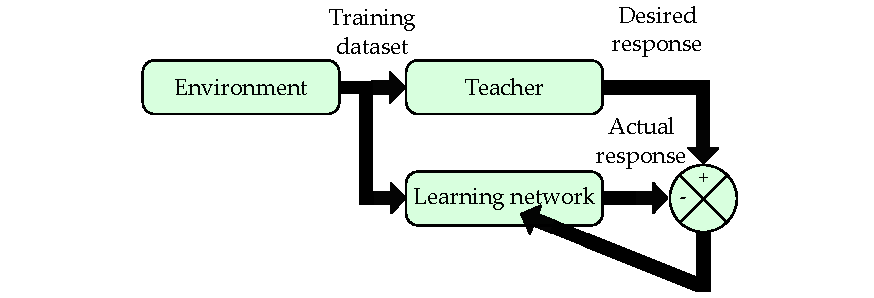
\includegraphics[width=\linewidth]{images/Ch2/fig7_SL2}} \quad
 	\caption[Block diagram of Supervised Learning (SL) with error-correction learning rule.]{Block diagram of Supervised Learning (SL) with error-correction learning rule.}\label{fig7_SL}
 \end{figure}
\subsection{System Identification}

One of the biggest applications of \ac{ML} is \ac{SI} of complex nonlinear dynamical systems whose dynamics cannot be represented by any mathematical model. \ac{SI} is deducing a mathematical description (a model) of a complex nonlinear dynamic system from a series of experimental measurements on the system. The motive for finding out the mathematical description of the dynamic systems are several. Some of them are the detection of faults, system simulation, the prediction for unknown input, and design of the control system. Often, \ac{SI} techniques are reliable when applying the laws of science becomes difficult for building a model. Depending upon the insight knowledge about the system, SI can be categorized into three types \cite{ljung1999system}:

\begin{itemize}
	\item Black-box modeling: \ac{SI} is fully based on the experimentally measured data, and no or minuscule knowledge about the dynamics of the system is available.
	\item Gray-box modeling: A certain degree of insight into the physical system is available, and it is used for the enhancement of empirical modeling.
	\item White-box modeling: Modelling a system by using its physical dynamics comes under the category of white-box modeling.
\end{itemize}

One of the biggest challenges in the field of complex nonlinear dynamical systems is finding out the underlying differential equations (partial) governing the system. The task here is to find out the DE of an unknown system from the observations made during the experiments. The data recorded during the experiments are in a time-series format so that a dynamical model can be built. Many different methods are discussed and proposed in the literature to achieve the required objective for the task. One of the methods for determining the \ac{DE} is \ac{ASR} \cite{Bongard2007automated, schmidt2009Distilling}. The main purpose of \ac{ASR} is to generate symbolic equations from time-series data of a nonlinear dynamic system \cite{Bongard2007automated}. \autoref{ddd}

\begin{equation}
\label{ddd}
{{y}^{(i)}}={{\mathbf{x}}^{(i)}}+{{\varepsilon }^{(i)}}
\end{equation}



\begin{align}
\label{GalerkinProj2}
\begin{split}
{{\mathbf x}(t)}\approx{\mathbf{\tilde{x}}}(t)={\mathbf\Psi}_{r}{\mathbf\Psi}_{r}^{T}{\mathbf{x}}(t)
\end{split}
\end{align}
